\documentclass{knittingpattern}
\usepackage[a4paper,total={7in, 10in}]{geometry}
\usepackage[table]{xcolor}
\usepackage{chemfig}
\usepackage{modiagram}
\usepackage{circuitikz}
\usepackage{tikz}
\usetikzlibrary{shapes,arrows,positioning}
\usepackage{xskak}
\usepackage{amssymb}
\usepackage{amsmath}
\usepackage{derivative}
\title{\color{blue}\centering\large\textbf{RAJIV GANDHI UNIVERSITY OF KNOWLEDGE TECHNOLOGIES,}}
\author{\color{blue}\centering\normalsize Basar (village \& mandal), Nirmal(District), Telangana State- 504107 }
\date{ \color{red}\centering \large \textbf{DEPARTMENT OF COMPUTER SCIENCE AND ENGINEERING.}}
\begin{document}
\maketitle
\hline
\vspace{0.5 cm}
\centering
\large{LATEX Assignment - 1(B192140)}
\\
\begin{flushleft}
\Large\textbf{Contents}
\section{Knitting Patterns}
\section{Chess Notation}
\section{Chemistry}
\subsection{Chemical Formulae}
\subsection{Molecular Orbital Diagrams}
\section{Electrical Circuits}
\section{Typesetting exams}
\end{flushleft}
\raggedright
This is an assignment. We are not sharing source code for this document- you'll have to look up the titles of each section (Overleaf is a great source) and try to replicate the features we demonstrate the best you can.\\
\medskip
Don't forget to give your ID when you submit the .file !\\
\medskip
We recommend you attempt this assignment online Overleaf editor for the most convenient work flow. The MacTex distribution has all packages installed.\\
\medskip
Some of the packages might give you troubles in your offline LATEX distribution, if so, you can switch over to Overleaf.\\
\bigskip
\bigskip
\centering
\fbox{\fbox { \parbox { 0.8\linewidth} {\centering{Your submissoin file should contain a zip containing}\\
\raggedright
1. Your source code (.tex file, .bib file) and supporting images, if any. The .tex file must be named ".tex"\\2.The pdf file, whose name must be ".pdf"\\3. The zip should be named ".zip". Consider your IIIT-B roll number and the assignment number.\\4. Same code should be in your Git Hub account.\\
5.B19XXXX.zip file need to be upload into (Server/Git-Hub rguktb-cse/your course will be specified in your lab.
}}}
\newpage
\usecounter{section}
\section{Knitting Patterns}
\raggedright
This class provides a very convenient way to introduce boxed diagrams. We are thus going to use our stock image a few more times. Also, it has a few features to make readable, however we can adapt them to make prettier documents for our purposes as well.
\\
\begin{figure}[h]
    \centering
    \setlength{\fboxsep}{15pt}
    \setlength{\fboxrule}{2pt}
\fbox{\includegraphics[scale=0.35]{graph.jpg}}
\end{figure}
\centering
\medskip
\fcolorbox{black}{yellow}{\parbox{10cm}{We have a way of highlighting important instructions.Feel free to choose whatever background and border colour you like. when you replicate these features ,but try to replicate dimensions as well as you can.}}
\\
\bigskip
{\rowcolors{1}{green!80!yellow!50}{green!70!yellow!40}
\begin{tabular}{ p{13cm} p{2cm} }
Courses & Credits\\
Introduction to Computer Programming & 6\\
Abstractions and Paradigms in Programming & 6\\
Abstractions and Paradigms in Programming Lab & 3\\
Data Structure and Algorithms & 6\\
Software Systems Lab & 8\\
\end{tabular}}\\
\bigskip
\centering
\fcolorbox{black}{teal}{\parbox{10cm}{\header{\begin{LARGE}\underline {NOTE:}\end{LARGE}}\\
This is a note. The above feature was introduced to typeset a sequence of knitting instructions.The first column is for the instruction, second for the number of stitches. But hey,it looks cool!}}\\
\bigskip
\bigskip
\intro{Look at the adjoining graph. Yes, you’ve seen it before. This time, it is side by side with a paragraph! And there’s a beautiful box around it! By default, this will be a quarter of the
width of the page. If you follow the hint that is the title of this section, you won’t have to type in cumbersome code to fit in images. Also, have you noticed that the pages are much
wider? Good luck!}{graph}
\newpage
\setcounter{section}{1} 
\section{Chess Notation}
\textbf{Adolf Anderson - Lionel Kieseritzky}\\
London, 1851
\\
\smallskip
\centering
\newchessgame
\hidemoves{1.e4 e5 2.f4 exf4 3.Bc4 Qh4+ 4.Kf1 b5 5.Bxb5 Nf6 6.Nf3 Qh6 7.d3 Nh5 8.Nh4 Qg5 9.Nf5 c6 10.g4 Nf6 11.Rg1 cxb5 12.h4 Qg6 13.h5 Qg5 14.Qf3 Ng8 15.Bxf4 Qf6 16.Nc3 Bc5 17.Nd5 Qxb2 18.Bd6}
\showboard
\\
\medskip
\raggedright
In this position, Black played \textbf{18...\symbishop $\times$ g1}, taking the rook.Had he opted for 18...\symqueen $\times$ a1, he would be better, but still in trouble .However, his choice allowed for a spectacular finish.\textbf{19 e5!} Blunting the Queen's protection of g7. \textbf{19...\symqueen $\times$ a1+.} Wgat else? The rool is en-prise. \textbf{20 \symking e2 \symknight a6.}This covers the c7 square, as white was threatening Mate in 2, example like 20...h6 21 \symknight Xg7+ \symking d8\hspace{2mm}22\hspace{2mm} \symbishop c7\char"0023. \textbf{21 \symknight Xg7+ \symking d8 22 \symqueen f6+!}\\
\medskip
\centering
\newchessgame
\hidemoves{1.e4 e5 2.f4 exf4 3.Bc4 Qh4+ 4.Kf1 b5 5.Bxb5 Nf6 6.Nf3 Qh6 7.d3 Nh5 8.Nh4 Qg5 9.Nf5 c6 10.g4 Nf6 11.Rg1 cxb5 12.h4 Qg6 13.h5 Qg5 14.Qf3 Ng8 15.Bxf4 Qf6 16.Nc3 Bc5 17.Nd5 Qxb2 18.Bd6 Bxg1 19.e5 Qxa1+ 20.Ke2 Na6 21.Nxg7+ Kd8 22.Qf6+ }
\showboard
\\
\medskip
\raggedright
A brilliant Queen sacrifice to deflect the knight on g8 that protects e7 \textbf{22... \symknight  $\times$f6 23 \symbishop e7\#}
\\
\medskip
\centering
\newchessgame
\hidemoves{1.e4 e5 2.f4 exf4 3.Bc4 Qh4+ 4.Kf1 b5 5.Bxb5 Nf6 6.Nf3 Qh6 7.d3 Nh5 8.Nh4 Qg5 9.Nf5 c6 10.g4 Nf6 11.Rg1 cxb5 12.h4 Qg6 13.h5 Qg5 14.Qf3 Ng8 15.Bxf4 Qf6 16.Nc3 Bc5 17.Nd5 Qxb2 18.Bd6 Bxg1 19.e5 Qxa1+ 20.Ke2 Na6 21.Nxg7+ Kd8 22.Qf6+ Nxf6 23.Be7#1-0}
\showboard
\\
\medskip
\raggedright
Chess enthusiasts will have immediately recognised this as the Immortal Game. Try typesetting this!
\\
\newpage
\setcounter{section}{2} 
\section{Chemistry}
\subsection{Chemical Formulae}
\centering
\chemfig{Cl-[:30]*6(-=(*6(-N=-=(-[:90]HN(-[:30](-[:90])-[:-30]-[:30]-[:-30]-[:30]N(-[:90]-[:30]-[:-30]OH)-[:-30]-[:30]))--))-=-=)}
\\
\medskip
\raggedright
This is the molecule hydroxychloroquine, that recently shot to fame as a proposed cure for COVID-19.Please draw it. This is a helpful Overleaf tutorial to help you get started.
\\
\subsection{Molecular Orbital Diagrams}
\centering
\begin{MOdiagram}[labels,names]
 \atom[N]{left}{
   2p = {0;up,up,up}
 }
 \atom[O]{right}{
   2p = {2;pair,up,up}
 }
 \molecule[NO]{
   2pMO  = {1.8,.4;pair,pair,pair,up} 
 }
\end{MOdiagram}
\\
\bigskip
\raggedright
You've probably mugged this up for JEE, and definately learnt more about this in CH 107.Draw the above molecular orbital diagram for nitric oxide.
\\
\newpage
\setcounter{section}{3} 
\section{Electrical Circuits}
\bigskip
\bigskip
\bigskip
\bigskip
\centering
\begin{circuitikz}[american voltages]
\draw
(0,0) 
to [short,*-*] (3,0)
to [short,-*] (6,0)
to [short,-*] (9,0) node [ground]
to [short,-*] (12,0)
to [short,-*] (13.5,0)
(3,0) to [short,-*,R,l=$R_2$,v=$V_B$] (3,3)
(0,3) to [short, *-*,C=$C_1$] (3,3)
(6,0) to [short, -*, R,l=$R_E$,v=$V_E$,i<_=$i_E$] (6,2.5) node [anchor=north west] {$V_C_E$}
(3,3) to [short,-,i_=$i_B$] (6,3)
(3,3) to [short,-,R=$R_1$] (3,6)
(6,3.5) to [short,-*,R=$R_L$,i<_=$i_C$] (6,6)
(3,6) to [short,-*,] (13.5,6)
(6,3) to [short,-*] (12,3)
(6,1.5) to [short,-] (9,1.5)
(9,1.5) to [short,-*,C=$C_2$] (9,0)
(0,0) to [open, v=$V_0sin(wt)$] (0,3)
(12,0) to [open, v=$V_o_u_t$] (12,4.5);
\draw (6,3) node [npn] (npn1)  {} 
 (npn1.base) node[anchor=north] {B}
 (npn1.collector) node[anchor=east] {C}
 (npn1.emitter) node[anchor=east] {E};
\end{circuitikz}
\\
\bigskip
\raggedright
If you recall JEE Physics, this is a circuit diagram of an npn transistor used as an amplifier. Try your best to match this
circuit. We have used the American voltages convention. It is alright if you can’t get the dimensions to match. What is
important is that you know how to use circuitikz to draw circuits with the components used above, and mark voltages and
currents.
\\
\setcounter{section}{4} 
\section{Typesetting exams}
\raggedright
Congratulations, you’re appointed as a TA for that course you loved last year. The prof, however, is busy with his research,
and wants you to typeset an exam. LATEX, with its exam class can help you do just that!
\smallskip

You’ll need to make a separate document, if you want to attempt this task. Your job is to imitate the exam.pdf that we
have provided.
\\
\newpage
%\rule{17.5cm}{0.3mm}
\begin{Large}
Maths
\end{Large}
\hspace{5.5cm}
\begin{Large}
Assignment
\end{Large}
\hspace{5.5cm}
\begin{Large}
IIITB \#
\end{Large}
\\
\hrulefill
\\
\bigskip
\textbf{problem 1.}Show that there exists no nontrivial unramified extensions of Q.
\\
\bigskip
\textbf{Solution:} If K/Q is a nontrivial number field, then | disc K | > 1. But then disc K has a prime factor so that some prime ramifies in K.\\
\bigskip
\textbf{Problem 2.} Complete the following:\\
\medskip
(a) How does one prove a cotheorem?\\
\medskip
(b) Compute \int cosx\hspace{1mm}dx.\\
\medskip
\\
(c) How does one square
\begin{pmatrix}
    a & b\\
    c & d\\
\end{pmatrix}\mathord{?}\\
\bigskip
\textbf{Solution:}\\
\medskip
(a) Use rollaries.\\
\medskip
(b) We have \\
\hspace{5cm}\int cosx\hspace{1mm}dx = sinx + C \hspace{4cm}(1)\\
\smallskip
\hspace{1cm} We can check (1):\\
\smallskip

\hspace{5cm}$\odv{}{x}$ (sinx + C) = cosx\\
\smallskip
(C) This is rouitne.\\
\bigskip
\textbf{Problem 3.} Prove that $\sqrt{2}$ is irrational.\\
\bigskip
\textit{Proof.} Assume that $\sqrt{2}$ = $\frac{a}{b}$, where a,b $\in$ Z. Without loss of generality, we may assume gcd(a,b) = \\
1.Then we have\\
\hspace{5cm}$\sqrt{2}$ = $\frac{a}{b}$\\
\smallskip
\hspace{5cm}${\sqrt{2}}^{2}$ = {($\frac{a}{b})$}^{2} \hspace{6cm}(2)\\
\smallskip
\hspace{5cm}2=$\frac{a^{2}}{b^{2}}$\\
\smallskip
\hspace{5cm}{a^{2}} = 2${b^{2}}$ \hspace{6.5cm}(3)
\medskip
But then from (3), we know that ${a^{2}}$ is even so that a is even. But then we must have \\
\medskip
\hspace{5cm} 2${a^{2}}$ =${b^{2}}$\\
\medskip
so that ${b^{2}}$ is even, implying b is even. But then gcd(a,b)$\ge$ 2, a contradiction.\\
\bigskip
\newpage
CSE 30151 Spring 2016 \hspace{11cm} Homework 2\\
\hrulefill\\
\bigskip
(b) \hspace{1cm}\\
\smallskip
\hspace{1cm}
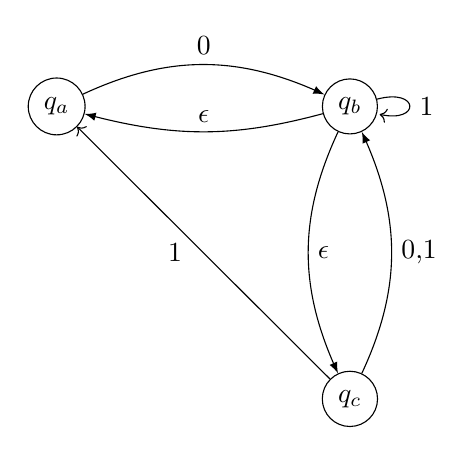
\begin{tikzpicture} [-latex,node distance=3cm]
\node [circle,draw] (a) {$q_{a}$};
\node[circle,draw] (b) [right=of a] {$q_{b}$};
\node[circle,draw] (c) [below=of b] {$q_{c}$};
\path (b) edge [bend right=-15] node [above] {$\epsilon$} (a);
\path (a) edge [bend left=25] node [above] {0} (b);
\path (b) edge [loop right] node [right]
{1} (a);
\path (b) edge [bend left=-25] node [right] {$\epsilon$} (c);
\path (c) edge [bend right=25] node [right] {0,1} (b);
\draw [->] (c)-- node[left=0.15cm] {1} (a);
\end{tikzpicture}
\\
\bigskip
4. \textbf{Solving puzzzle \#1} In class, we did three puzzles, the first of which is equivalent to
finite automata. In general, a puzzle of this type has a frame like this (but possibly
with more/fewer squares and different colors):\\
\bigskip
\bigskip
\centering
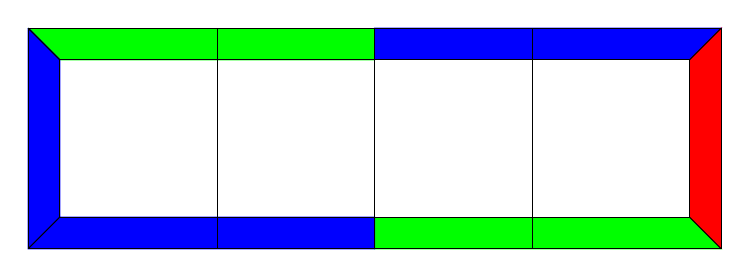
\begin{tikzpicture}

\filldraw[green](-0.4,2.4)--(0,2)--(4,2)--(4,2.4);
\filldraw[green](4,0)--(4,-0.4)--(8.4,-0.4)--(8,0);
\filldraw[blue](4,2)--(4,2.4)--(8.4,2.4)--(8,2);
\filldraw[blue](-0.4,2.4)--(0,2)--(0,0)--(4,0)--(4,-0.4)--(-0.4,-0.4)--(-0.4,2.4);
\filldraw[red](8,0)--(8,2)--(8.4,2.4)--(8.4,-0.4);
\draw (0,0) -- (2,0) -- (2,2) -- (0,2) -- (0,0);
\draw (2,2) -- (4,2) -- (4,0) -- (2,0);
\draw (4,2) -- (6,2) -- (6,0) -- (4,0);
\draw (6,2) -- (8,2) -- (8,0) --(6,0);
\draw (0,0) -- (-0.4,-0.4);
\draw (0,2) -- (-0.4,2.4);
\draw (-0.4,2.4) -- (-0.4,-0.4);
\draw (2,2) -- (2,2.4);
\draw (4,2) -- (4,2.4);
\draw (6,2) -- (6,2.4);
\draw (8,2) -- (8.4,2.4);
\draw(-0.4,2.4) -- (8.4,2.4);
\draw (2,0) -- (2,-0.4);
\draw (4,0) -- (4,-0.4);
\draw (6,0) --( 6,-0.4); 
\draw (8,0) -- (8.4,-0.4);
\draw (-0.4,-0.4) -- (8.4 ,-0.4);
\draw (8.4,-0.4) --(8.4,2.4);
\end{tikzpicture}

\\
\bigskip
\bigskip
And a finite set of tiles like this (but possibly with more/fewer tiles and different colors):\\
\bigskip
\bigskip
\centering
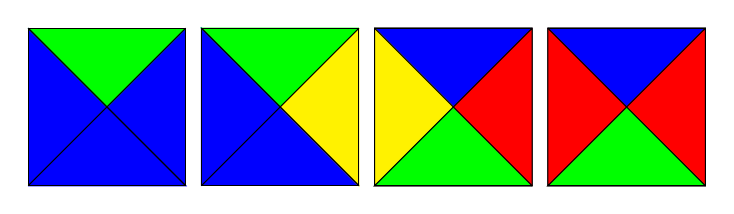
\begin{tikzpicture}

\draw (0,0) -- (2,0) -- (2,2) -- (0,2) -- (0,0);

\filldraw[blue] (0,0) -- (2,0) -- (0,2) ;
\filldraw[blue] (0,0) -- (2,0) -- (2,2) ;
\filldraw[green] (0,2) -- (1,1) -- (2,2);
\draw (0,0) -- (2,2);
\draw (2,0) -- (0,2);
\draw (0,0) -- (2,0) -- (2,2) -- (0,2) -- (0,0);

\draw (2.2,0) -- (2.2,2) --(4.2 ,2) -- (4.2,0)--(2.2,0)  ;
\filldraw[blue] (2.2,0) -- (2.2,2) --(4.2,0) ;
\filldraw[yellow](3.2,1)--(4.2,0)--(4.2,2);
\filldraw[green](3.2,1)--(2.2,2)--(4.2,2);
\draw(2.2,0)--(2.2,2)--(4.2,2)--(4.2,0)--(2.2,0);
\draw (4.2,0)-- (2.2,2);
\draw(2.2,0)--(4.2,2);

\draw (4.4,0)-- (4.4,2) -- (6.4,2) -- (6.4,0)--(4.4,0)--(6.4,2) ;
\draw (6.4,0)-- (4.4,2);
\filldraw[blue] (4.4,2) -- (5.4,1) --(6.4,2) ;
\filldraw[yellow](4.4,0)--(5.4,1)--(4.4,2);
\filldraw[green](4.4,0)--(5.4,1)--(6.4,0);
\filldraw[red](6.4,2)--(5.4,1)--(6.4,0);
\draw (4.4,0)-- (4.4,2) -- (6.4,2) -- (6.4,0)--(4.4,0)--(6.4,2) ;
\draw (6.4,0)-- (4.4,2);



\draw (6.6,0)-- (6.6,2) -- (8.6,2)-- (8.6,0)--(6.6,0)--(8.6,2) ;
\draw (8.6,0) --((6.6,2);
\filldraw[blue] (6.6,2) -- (7.6,1) --(8.6,2) ;
\filldraw[red](8.6,0)--(7.6,1)--(8.6,2);
\filldraw[green](6.6,0)--(7.6,1)--(8.6,0);
\filldraw[red](6.6,2)--(7.6,1)--(6.6,0);

\draw (6.6,0)-- (6.6,2) -- (8.6,2)-- (8.6,0)--(6.6,0)--(8.6,2) ;
\draw (8.6,0) --((6.6,2);
\end{tikzpicture}


\bigskip
\bigskip
\raggedright
The title must be arranged so that adjacent areas have matching colors. There is an unlimited number of copies of each tile.\\
\bigskip
(a) \hspace{1mm} Show how every puzzle of this type can be converted into a finite automaton \textit{M} and a string $\omega$ such that \textit{M} accepts  $\omega$ if and only if the puzzle has a solution. \\
\medskip
(b) \hspace{1mm} Apply your construction to the above instance.\\
\medskip
(c) \hspace{1mm} Briefly describe how this gives an \textit{O(n)} algorithm for solving puzzles of this type.\\


\end{document}
